\section{Results}
    The initial plan was to carry the testing out in a testing bench provisioned by the university. Notwithstanding, due to external technical constraints, it end up not being possible. I finally decided to conduct all the tests from my machines.
    Tests were performed in my local cluster. The following tables lists the physical devices and virtualized machines used. The virtualization software used is VMWare Workstation 16 Pro.
    
    \subsection{Testing environment and setup}
        List of physical devices used in the test:
        
        \begin{itemize}
            \item Desktop Personal Computer
            \item Laptop
            \item Raspberry Pi 4 (4 GB)
            \item Raspberry Pi Zero W
        \end{itemize}
        
        The following sub-sections enumerate the components of the Yako platform, mentioned in section \ref{section:backend}, and the location of these services.
        
        \subsubsection{Apache Zookeeper}
            ZK was run on my physical laptop with a x86\_64 Intel i7-8550U CPU, operating under a Linux Kali rolling distribution. The service was available at the default port established in the configuration file \ref{code:zoo_conf}.
            
            \begin{table}[H]
                \centering
                \caption{Apache Zookeeper service discovery service location}
                \label{tab:test_zk}
                \begin{tabular}{|l|l|l|l|}
                    \hline
                    \rowcolor[HTML]{C0C0C0}
                    \textbf{Device} & \textbf{IP}  & \textbf{Port} & \textbf{OS} \\\hline
                    Laptop & 192.168.1.41 & 2181 & Kali Linux Rolling 2022.1 \\ \hline
                \end{tabular}
            \end{table}
        
        \subsubsection{Mosquitto MQTT Broker}
            The MQTT broker was also run under the same physical device as ZK. The service is exposed at the port defined in snippet \ref{code:moquitto_conf}.
            
            \begin{table}[H]
                \centering
                \caption{Mosquitto MQTT Broker service location}
                \label{tab:test_mqtt}
                \begin{tabular}{|l|l|l|l|}
                    \hline
                    \rowcolor[HTML]{C0C0C0}
                    \textbf{Device} & \textbf{IP}  & \textbf{Port} & \textbf{OS} \\\hline
                    Laptop & 192.168.1.41 & 8002 & Kali Linux Rolling 2022.1 \\ \hline
                \end{tabular}
            \end{table}
        
        \subsubsection{YakoMaster}
            The YakoMaster orchestrator service was available on the same laptop. All, this and previously mentioned, services are running in the same physical device because of the limited testing devices available. Nevertheless, in a production environment, these could be deployed and ran in different physical machines. To all intents and purposes, it is advised to do so, to avoid SPOF \cite{vmware_inc_what_nodate} and increase security.
            
            \begin{table}[H]
                \centering
                \caption{YakoMaster and YakoAPI service location}
                \label{tab:test_yakomasters}
                \begin{tabularx}{\linewidth}{|l|l|l|X|l|l|X|}
                    \hline
                    \rowcolor[HTML]{C0C0C0}
                    \textbf{Device} & \textbf{IP} & \textbf{Port} & \textbf{OS} & \textbf{CPU} & \textbf{RAM} & \textbf{GPU} \\ \hline
                    Laptop & 192.168.1.41 & 8001 & Kali Rolling 2022.1 & Intel i7-8550U & 16GB & NVIDIA GTX 1050 \\ \hline
                \end{tabularx}
            \end{table}
        
        \subsubsection{YakoAgents}
            All the available YakoAgents were VMs, virtualized in both my desktop workstation and my portable computer.
            
            \begin{table}[H]
                \centering
                \caption{YakoAgents services locations}
                \label{tab:test_yakoagents}
                \begin{tabularx}{\linewidth}{|l|l|l|X|X|l|}
                    \hline
                    \rowcolor[HTML]{C0C0C0}
                    \textbf{Device} & \textbf{IP} & \textbf{Port} & \textbf{OS} & \textbf{CPU} & \textbf{RAM} \\ \hline
                    PC & 192.168.1.44 & 8001 & Ubuntu 20.04.4 LTS (Focal Fossa) & AMD Ryzen 7 3700X (2 Cores) & 4GB \\ \hline
                    PC & 192.168.1.45 & 8002 & CentOS Stream 8 & AMD Ryzen 7 3700X (1 Core) & 1GB \\ \hline
                    PC & 192.168.1.46 & 8003 & Ubuntu 21.10 (Impish Indri) & AMD Ryzen 7 3700X (4 Cores) & 8GB \\ \hline
                    PC & 192.168.1.47 & 8004 & CentOS Stream 9 & AMD Ryzen 7 3700X (4 Cores) & 12GB \\ \hline
                    
                    Laptop & 192.168.145.128 & 8005 & Ubuntu 20.04.4 LTS (Focal Fossa) & Intel(R) Core(TM) i7-8550U CPU @ 1.80GHz (2 Cores) &  4GB \\ \hline
                    Laptop & 192.168.145.129 & 8006 & CentOS Stream 8 & Intel(R) Core(TM) i7-8550U CPU @ 1.80GHz (1 Core) & 1GB \\ \hline
                    Laptop & 192.168.145.130 & 8007 & Ubuntu 21.10 (Impish Indri) & Intel(R) Core(TM) i7-8550U CPU @ 1.80GHz (4 Cores) & 8GB \\ \hline
                \end{tabularx}
            \end{table}
            
            The heterogeneity components of these environments were elevated as much as possible, by setting different hardware configurations (CPU cores, RAM and Secondary Memory [HDD, SSD, NVMe SSD]), and differing software configurations. The OSes used in these machines are different versions of Linux Ubuntu (20.04 LTS and 21.10) and CentOS (Stream 8 and Stream 9).
        
        \subsubsection{YakoAgents (IoT)}
            On the other hand, YakoAgents (IoT) were physical Raspberry Pis devices. The Pi 4 was connected to the network through a gigabit switch and the Pi Zero W through a wireless connection (802.11 b/g/n) up to 600 Mbps. The more capable device booted from a 2.0 USB device while the other was ran from a micro SD (see Figure \ref{fig:test_iot_devices}).
            
            \begin{table}[H]
                \centering
                \caption{YakoAgents (IoT) services locations}
                \label{tab:test_yakoagentsiot}
                \begin{tabularx}{\linewidth}{|X|l|l|X|X|l|X|}
                    \hline
                    \rowcolor[HTML]{C0C0C0}
                    \textbf{Device} & \textbf{IP} & \textbf{Port} & \textbf{OS} & \textbf{CPU} & \textbf{RAM} \\ \hline
                    Raspberry Pi 4 & 192.168.1.35 & 8001 & Raspbian 10 (Buster) 32-bits & ARMv7 processor rev 3 (v7l) & 4GB\\ \hline
                    Raspberry Pi Zero W & 192.168.1.76 & 8002 & Raspbian 10 (Buster) 32-bits & ARMv6 processor rev 7 (v6l) & 512MB \\ \hline
                \end{tabularx}
            \end{table}
            
            \begin{figure}[H]
                \centering
                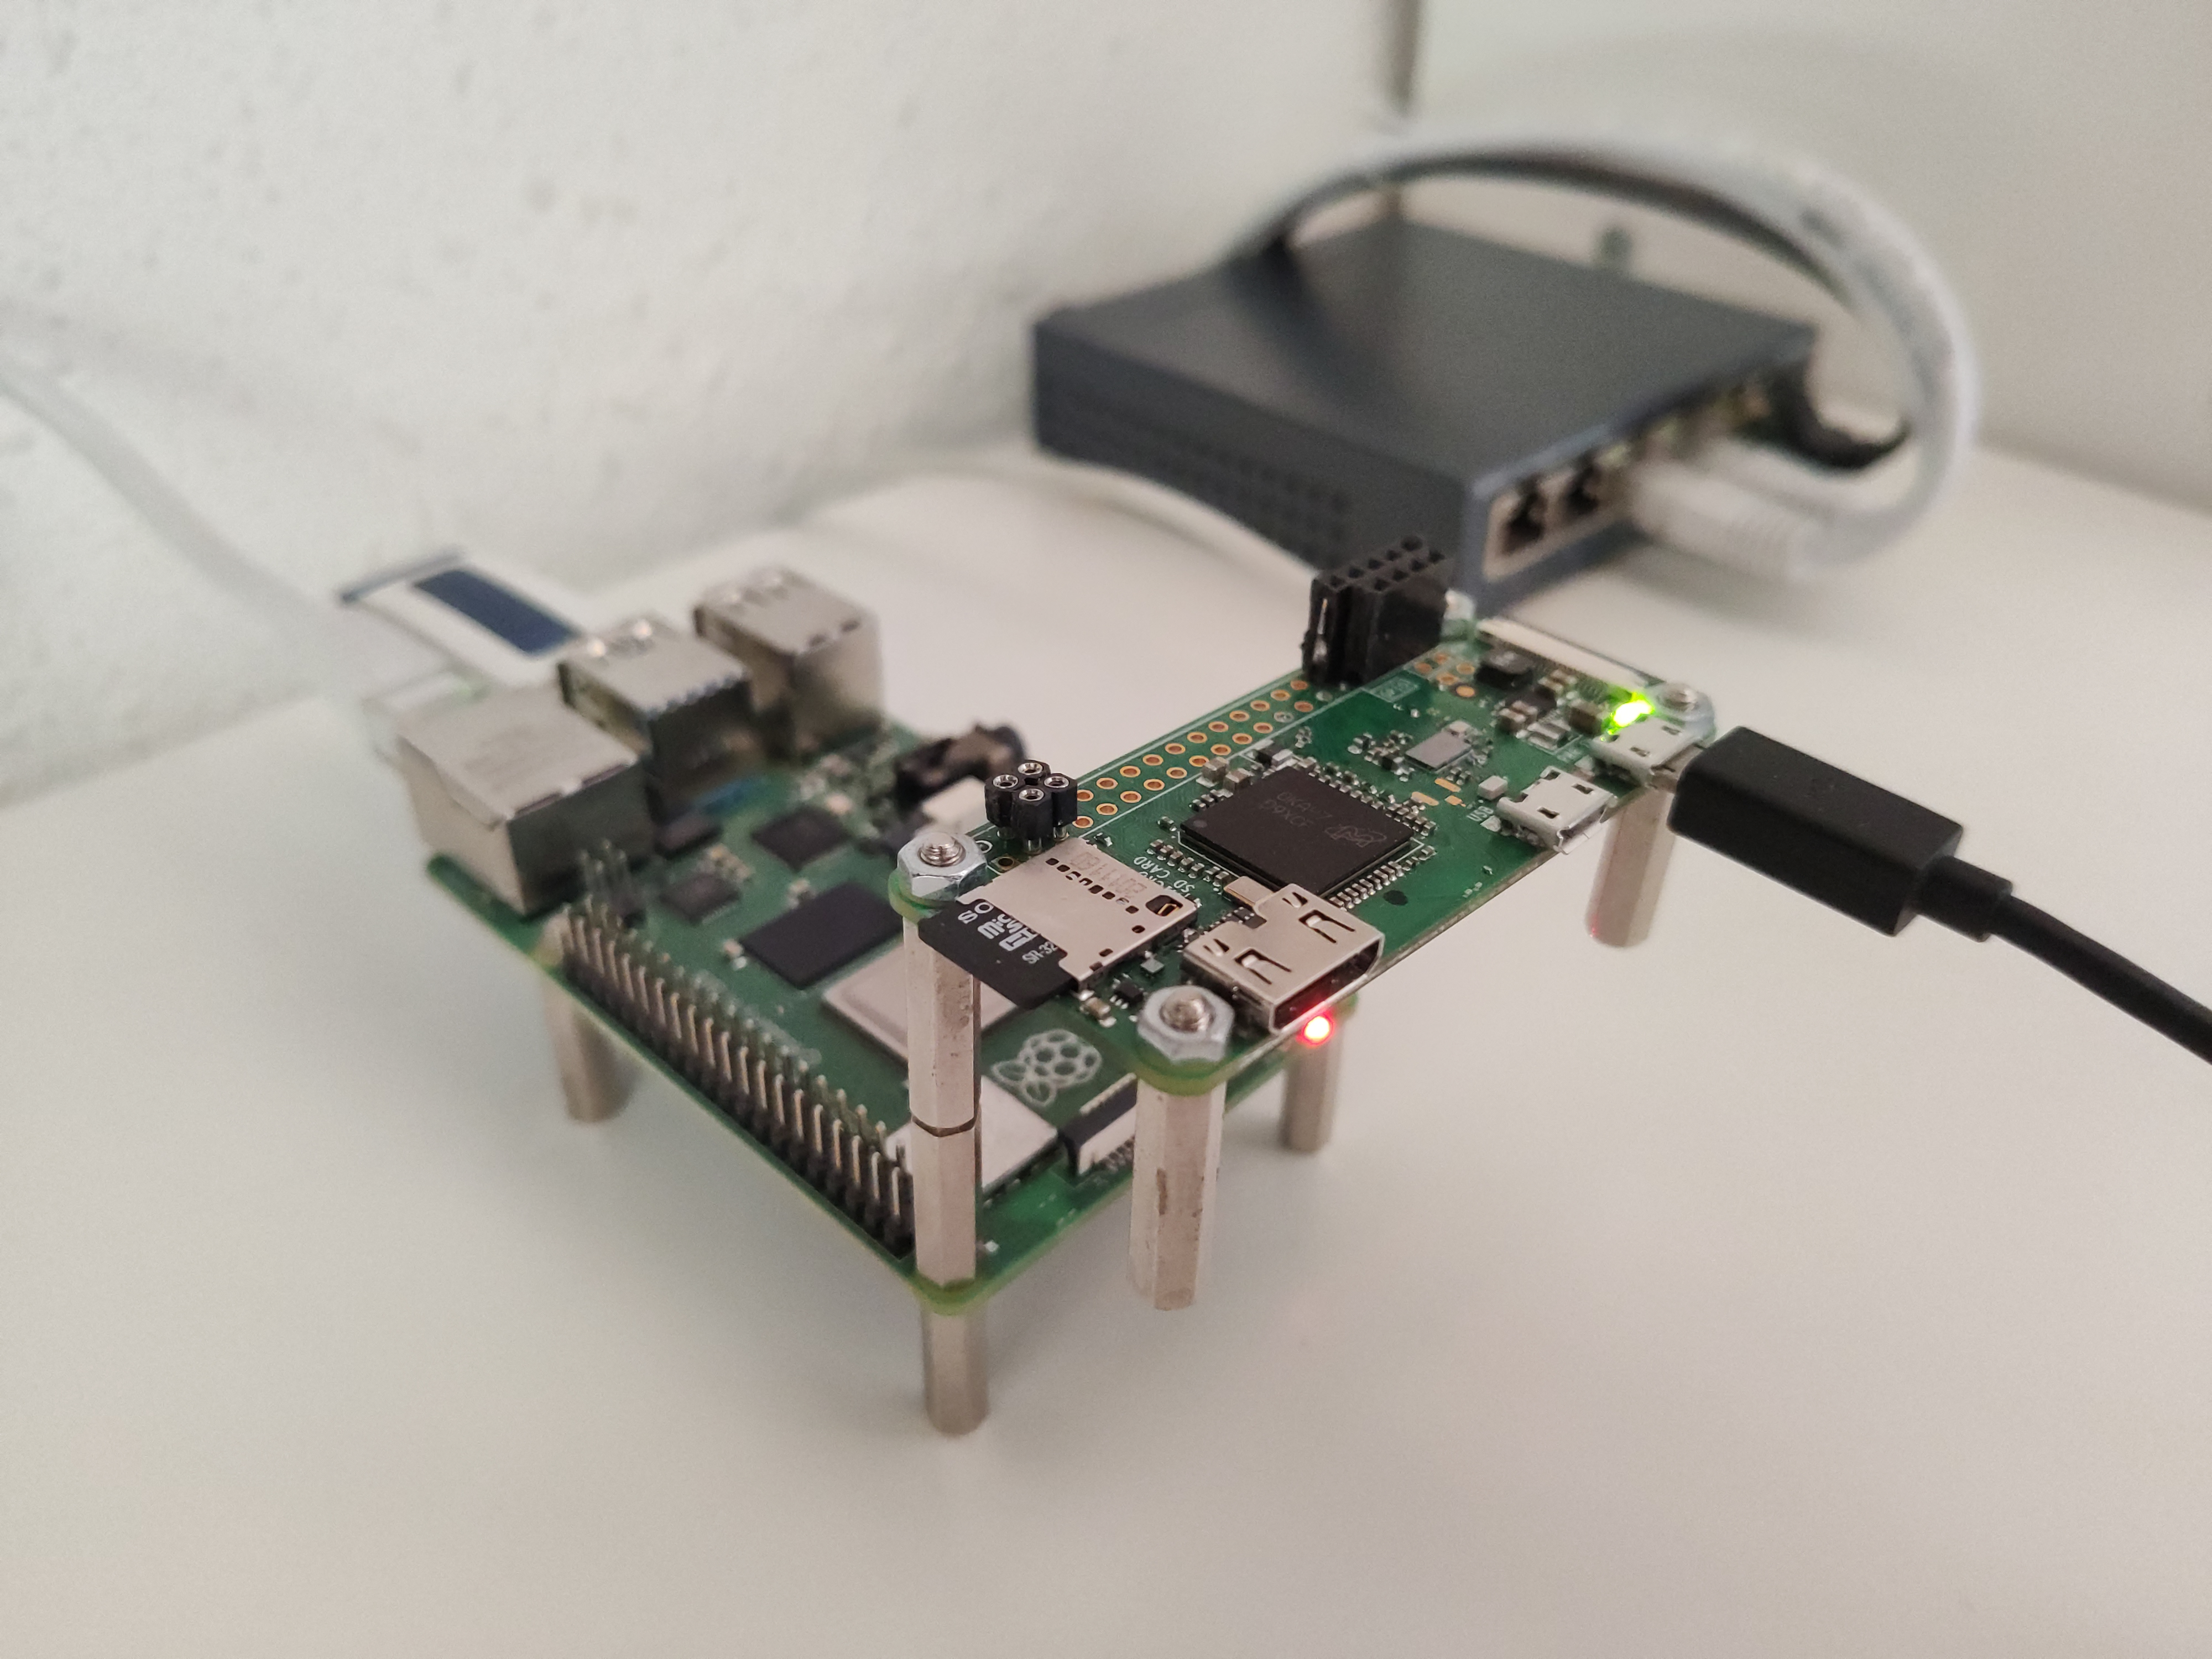
\includegraphics[width=0.8\linewidth]{Results/test_iot_devices.jpg}
                \caption{YakoAgents (IoT) Raspberry Pi physical devices}
                \label{fig:test_iot_devices}
            \end{figure}
        
        \subsubsection{YakoUI}
            For this specific test shown in the figure \ref{fig:test_yakoui_windows}, the front-end application was run on a Windows 11 device. However, previous testings were performed on Kali Linux. The web version is also accessible from a web browser at the hosting device served at port 8080 (see Figure \ref{fig:test_yakoui_web}). The service port can be configured on Webpack server configuration. In a production environment this should be on port 80 (HTTP) or 443 (HTTPS).
            \begin{table}[H]
                \centering
                \caption{YakoUI front-end application location}
                \label{tab:test_yakoagentsiot}
                \begin{tabularx}{\linewidth}{|l|l|X|X|l|X|}
                    \hline
                    \rowcolor[HTML]{C0C0C0}
                    \textbf{Device} & \textbf{IP} & \textbf{OS} \\\hline
                    PC & 192.168.1.37 & Windows 11 Insider Preview 25126.1000 (rs\_prerelease)  \\ \hline
                \end{tabularx}
            \end{table}
            
            \begin{figure}[H]
                \centering
                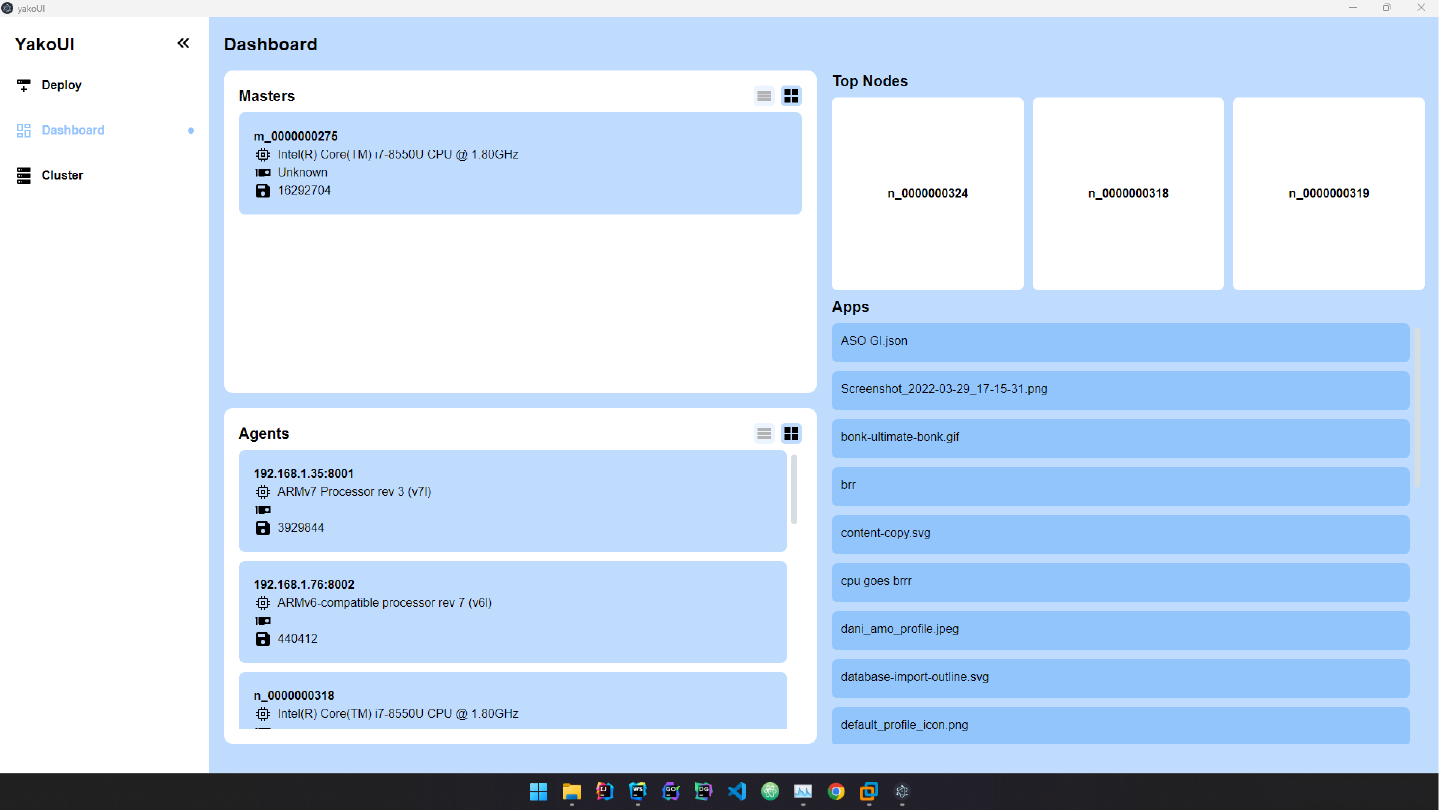
\includegraphics[width=0.9\linewidth]{Results/test_yakoui_windows.png}
                \caption{YakoUI application running on a Windows 11 device}
                \label{fig:test_yakoui_windows}
            \end{figure}
            
            \begin{figure}[H]
                \centering
                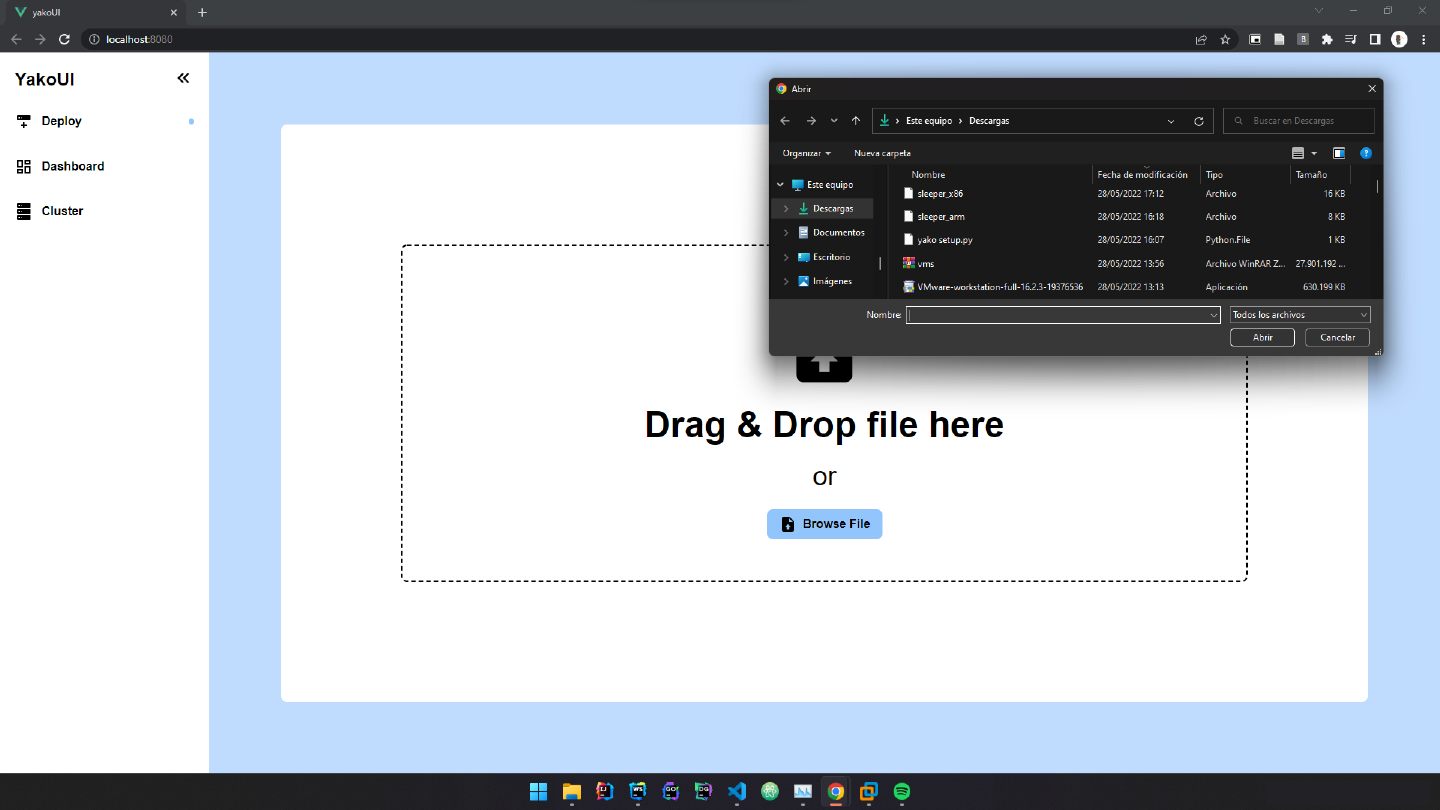
\includegraphics[width=0.9\linewidth]{Results/test_yakoui_web.png}
                \caption{YakoUI application accessed from the web}
                \label{fig:test_yakoui_web}
            \end{figure}
    
    \subsection{Testing procedure}
        On application startup the first view shown is the Upload application page. Before the upload of an executable to the system, agent devices must be connected first, figure \ref{fig:test_no_agents}. During the testing stage, laptop VM YakoAgents were connected first, figure \ref{fig:test_agent_connect_1}. Physical Raspberries YakoAgents (IoT), figure \ref{fig:test_agent_iot_connect}, were added following the prior devices connections. Lastly, PC VM YakoAgents were included to the platform as shown in \ref{fig:test_agent_connect_2}.
        
        \begin{figure}[H]
            \begin{subfigure}{0.5\textwidth}
                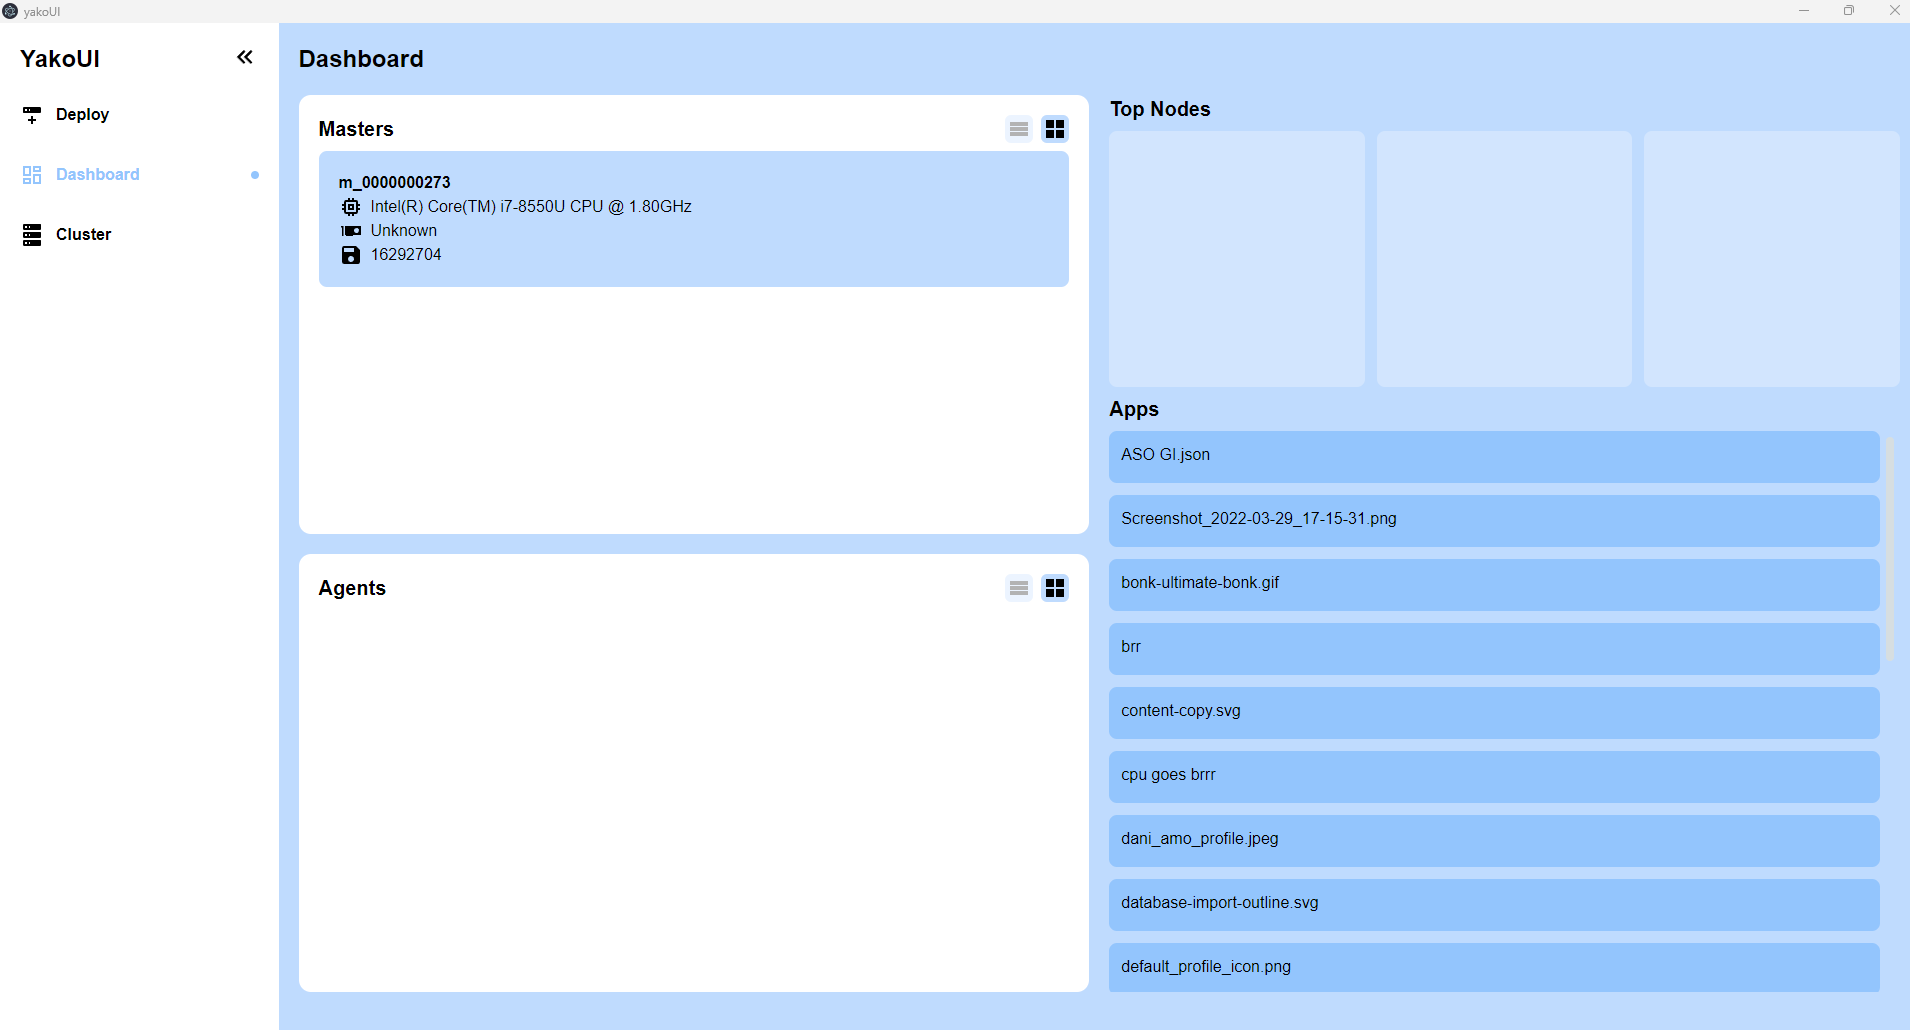
\includegraphics[width=\textwidth]{Images/Results/test_no_agents.png}
                \subcaption{No agents connected}
                \label{fig:test_no_agents}
            \end{subfigure}
            \begin{subfigure}{0.5\textwidth}
                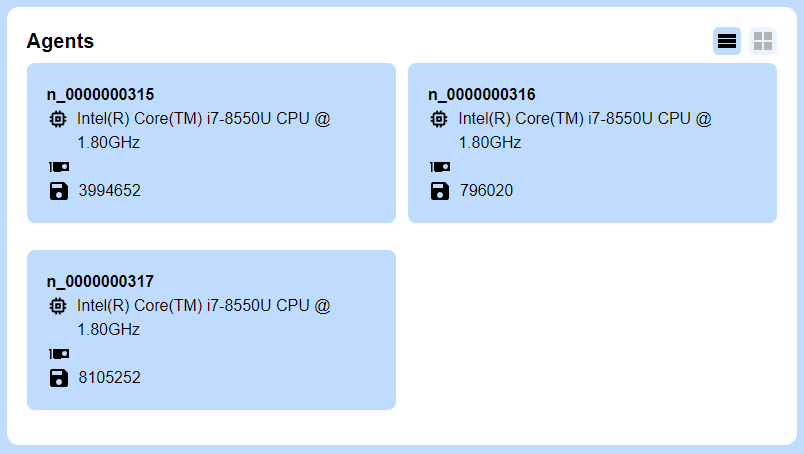
\includegraphics[width=\textwidth]{Images/Results/test_agent_connect_1.png}
                \subcaption{Laptop YakoAgent connections}
                \label{fig:test_agent_connect_1}
            \end{subfigure}
            \vskip\baselineskip
            \begin{subfigure}{0.5\textwidth}
                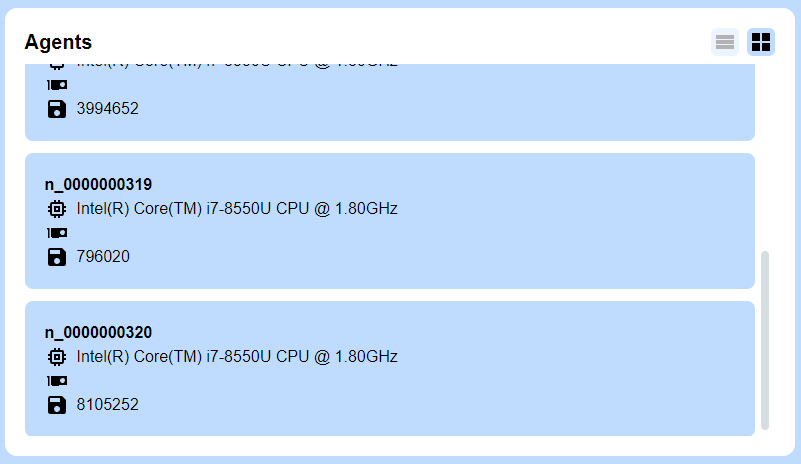
\includegraphics[width=\textwidth]{Images/Results/test_agent_iot_connect.png}
                \subcaption{Pis YakoAgent (IoT) connections}
                \label{fig:test_agent_iot_connect}
            \end{subfigure}
            \begin{subfigure}{0.5\textwidth}
                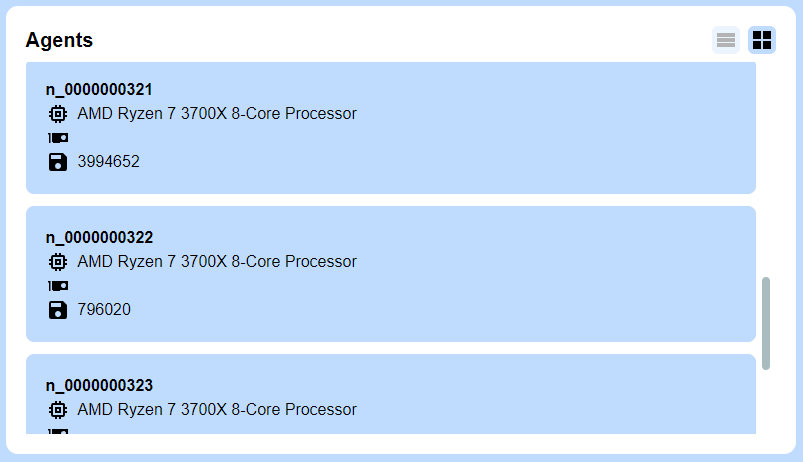
\includegraphics[width=\textwidth]{Images/Results/test_agent_connect_2.png}
                \subcaption{PC YakoAgent connections}
                \label{fig:test_agent_connect_2}
            \end{subfigure}
            \caption{YakoAgent and YakoAgent (IoT) devices connections}
            \label{fig:test_agents_connection}
        \end{figure}
        
        
        Figure \ref{fig:test_cluster_graph} illustrates the resulting diagram of all connected devices in the platform from the Cluster graph view of the front-end application. The root node is the YakoMaster orchestrator, the first column after that are the IoT devices. The middle column are the 3 laptop VMs agents, and the last column are the 4 PC VMs.
        
        \begin{figure}[H]
            \centering
            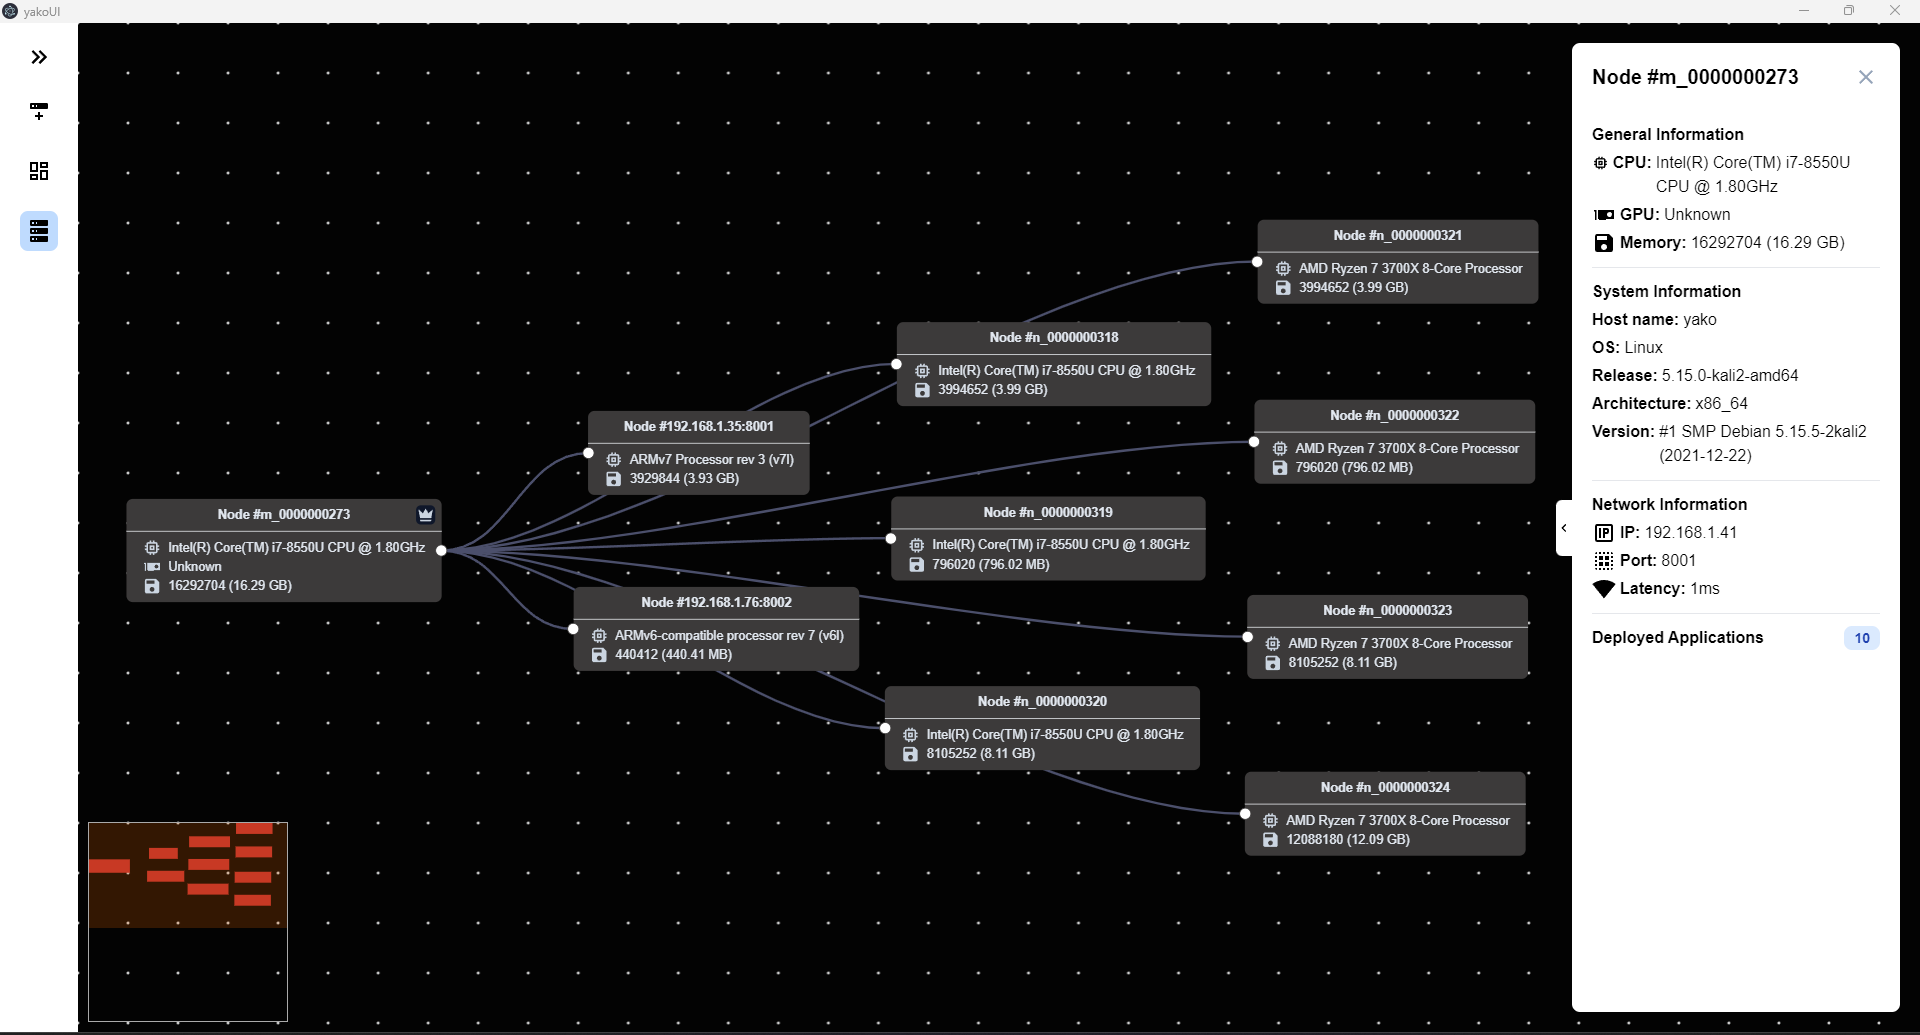
\includegraphics[width=\linewidth]{Results/test_cluster_graph.png}
            \caption{Test bed cluster graph}
            \label{fig:test_cluster_graph}
        \end{figure}
        
        \subsubsection{YakoAgent (IoT) Application deployment}
            The testing program, sleeper.c (see source code \ref{code:sleeper_once}) was compiled into a binary executable called sleeper\_arm. This small executable prints on a standard output sleeps for 5 seconds and finishes its process. The resulting compiled executable is platform and architecture dependent and should be taken into consideration. An application that has been compiled for a traditional desktop grade CPU architecture, like x86\_64 would not work in an IoT ARM based device. The bits of the OS should also be taken into consideration. Currently, Yako platform does not support architecture and platform search, but it could be added in the future as a filter in the upload form.
            
            \begin{code}
                \inputminted[
                    frame=lines,
                    framesep=2mm,
                    baselinestretch=1,
                    bgcolor=LightGray,
                    fontsize=\footnotesize,
                    escapeinside=||,
                    breaklines=true,
                    linenos
                ]{c}{Code/Results/sleeper_once.c}
                \caption{Sleeper Once}
                \label{code:sleeper_once}
            \end{code}
            
            Running the "file" command on the compiled versions of sleeper.c for x86\_64 (see figure \ref{code:file_sleeper_x86_64}) and ARM (see figure \ref{code:file_sleeper_arm}) results in differing properties, despite the fact that both binaries are originated from the same source code.
            
            \begin{code}
                \inputminted[
                    frame=lines,
                    framesep=2mm,
                    baselinestretch=1,
                    bgcolor=LightGray,
                    fontsize=\footnotesize,
                    breaklines=true,
                    linenos
                ]{shell}{Code/Results/file_sleeper_x86_64.sh}
                \caption{64-bits Sleeper binary for x\_86\_64 "file" command output}
                \label{code:file_sleeper_x86_64}
            \end{code}
            
            \begin{code}
                \inputminted[
                    frame=lines,
                    framesep=2mm,
                    baselinestretch=1,
                    bgcolor=LightGray,
                    fontsize=\footnotesize,
                    breaklines=true,
                    linenos
                ]{shell}{Code/Results/file_sleeper_arm.sh}
                \caption{32-bits Sleeper binary for ARM "file" command output}
                \label{code:file_sleeper_arm}
            \end{code}
            
            \begin{figure}[H]
                \centering
                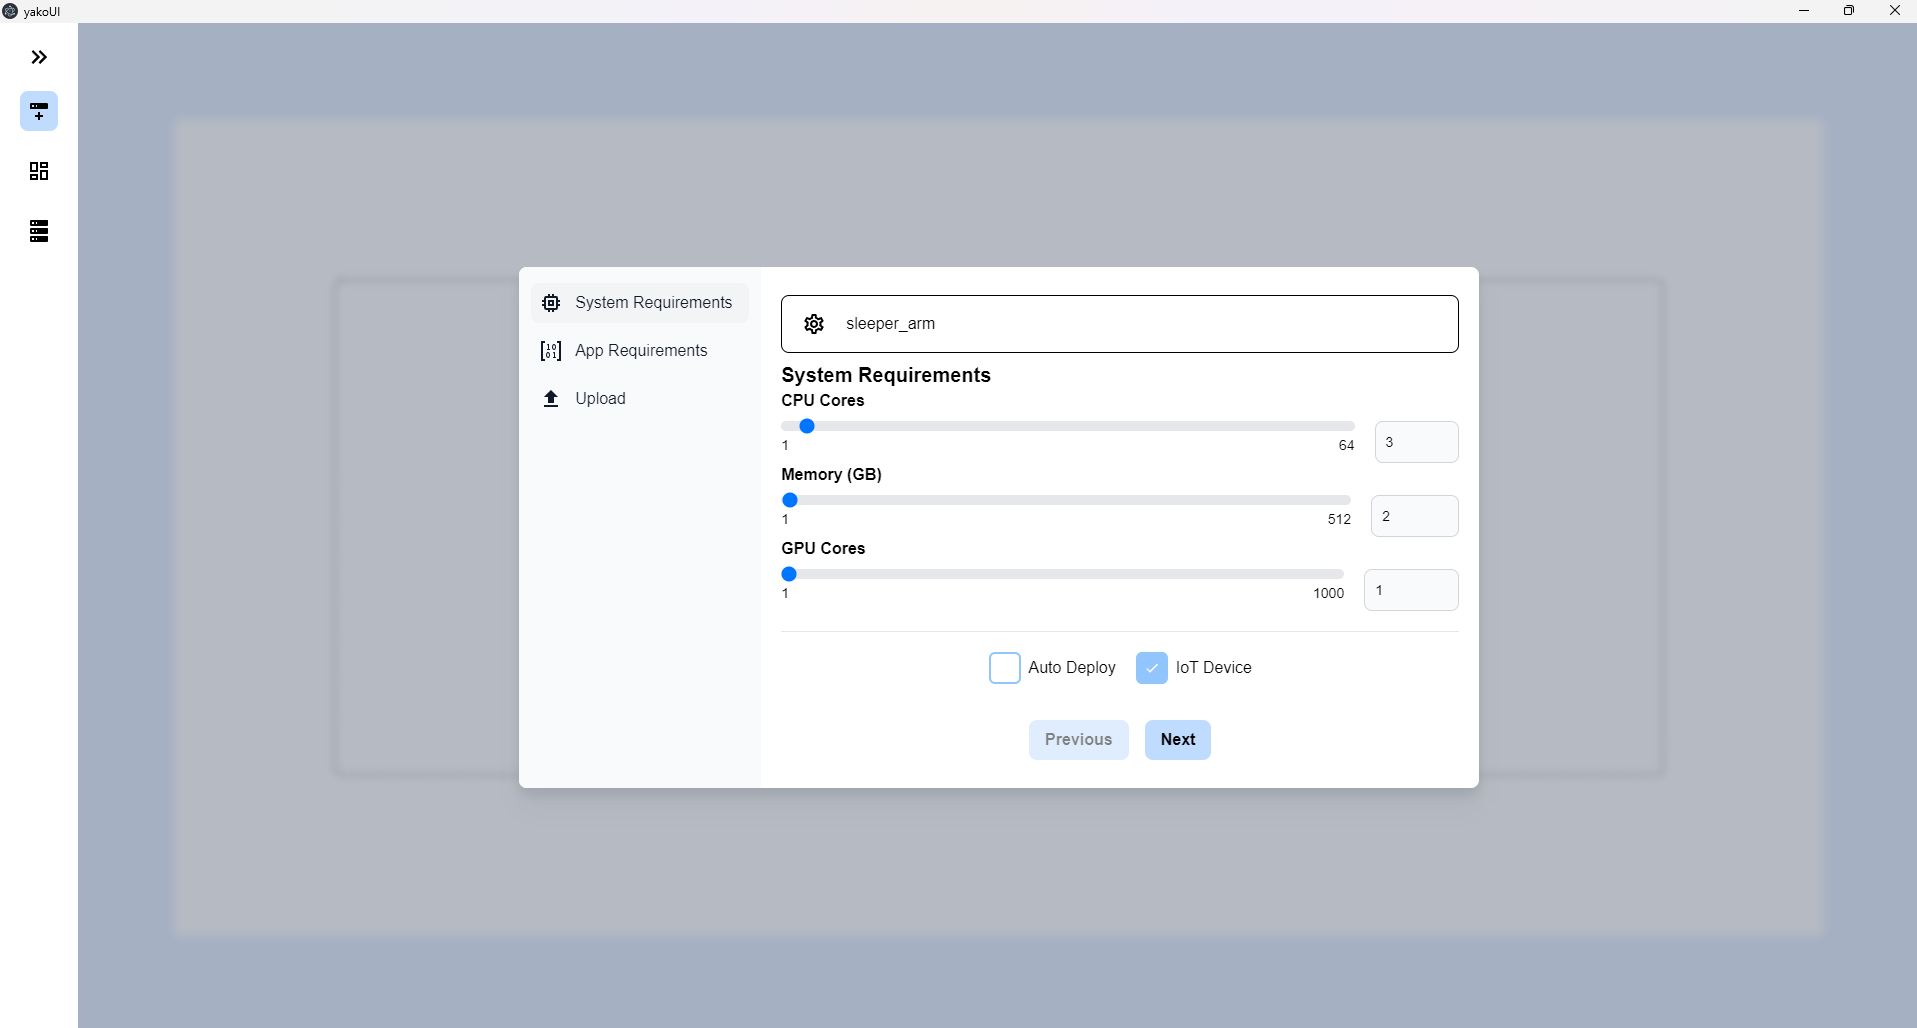
\includegraphics[width=\linewidth]{Results/test_agent_iot_form.png}
                \caption{System requirements form to deploy a 32-bits app to ARM based IoT devices}
                \label{fig:test_agent_iot_form}
            \end{figure}
            
            Back to the Upload Application page, the executable was loaded in the front-end application. Following, the system requirements form was presented and the selection was an IoT node that should have 3 CPU cores and 2 GB of available RAM.
            
            \begin{figure}[H]
                \centering
                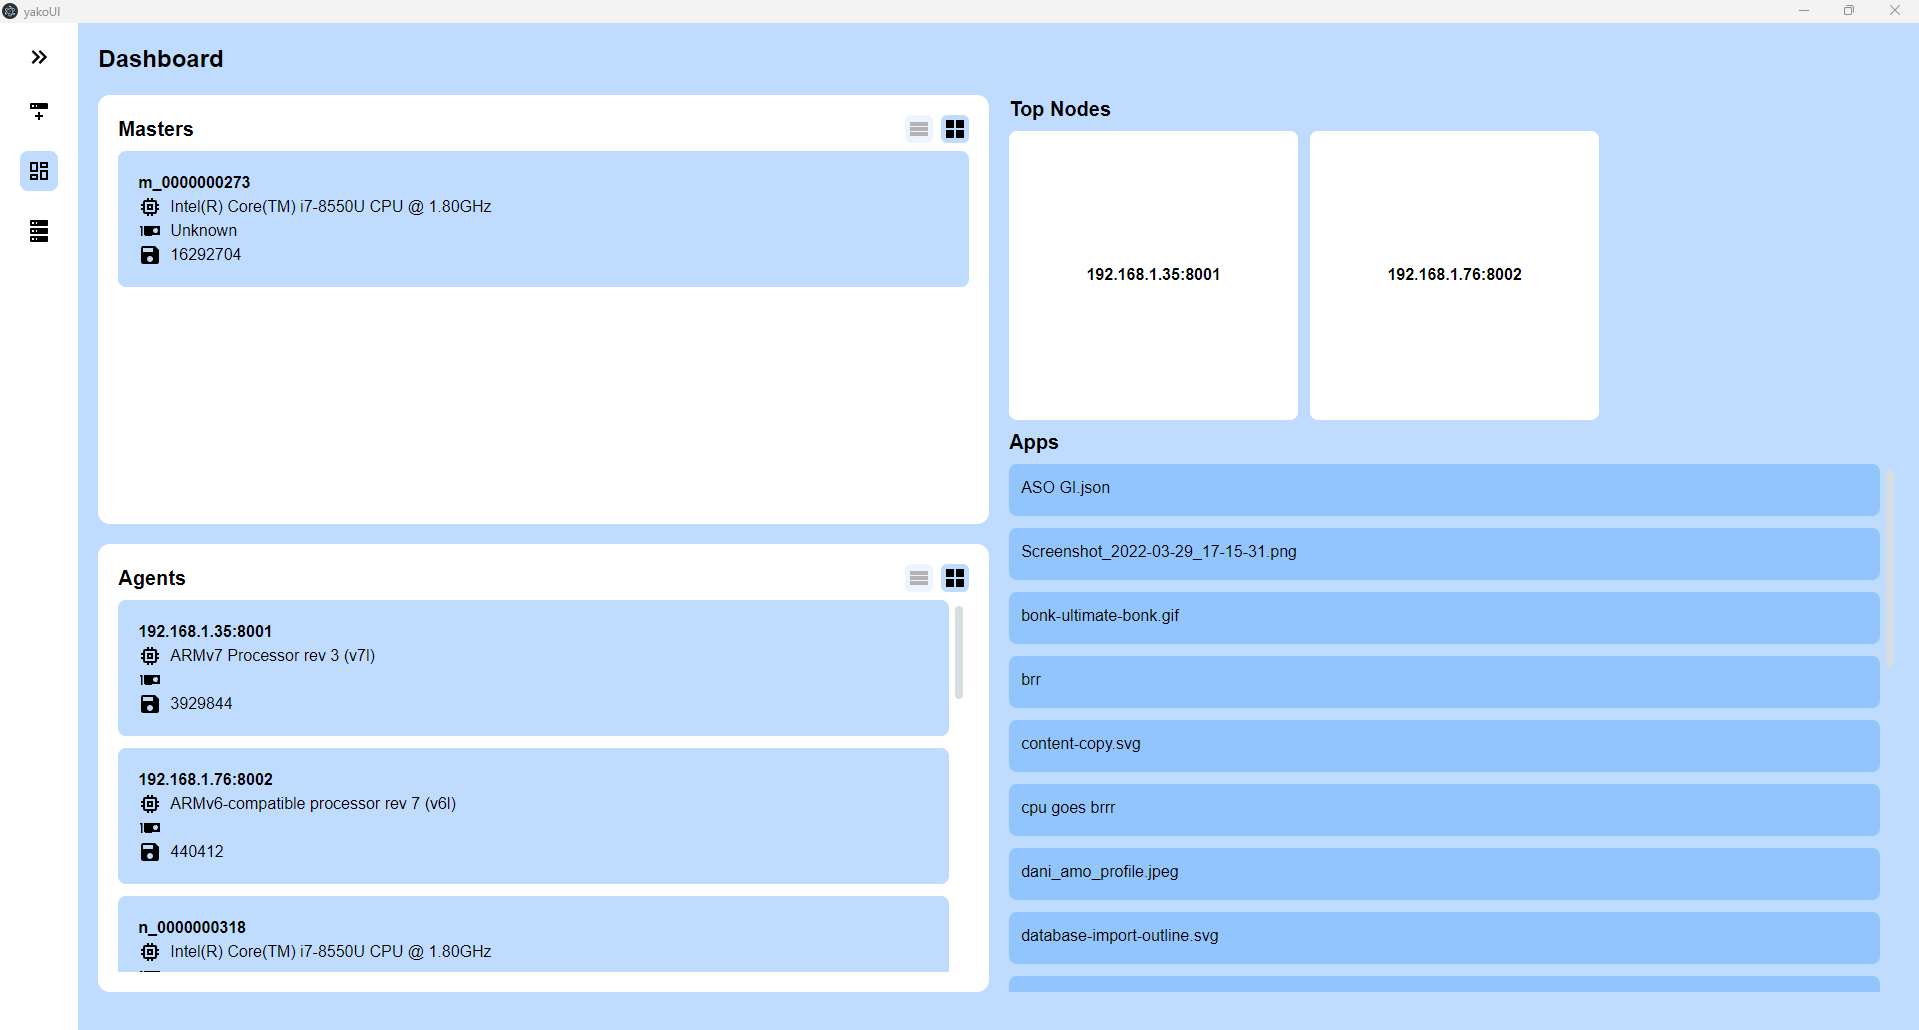
\includegraphics[width=\linewidth]{Results/test_agent_iot_top_nodes.png}
                \caption{Top IoT ARM based nodes for a 32-bits app complying the specified system requirements}
                \label{fig:test_agent_iot_top_nodes}
            \end{figure}
            
            After the upload of the application and requisites form, YakoMaster the orchestrator searches for the most suitable agent and presents these back to the front-end application Dashboard page. For this particular test, the application was deployed to the node residing at 192.168.145.35, the Raspberry Pi 4 which has 4GB of RAM and 4 CPU cores, since the other IoT device had lower specifications.
            
            \begin{figure}[H]
                \centering
                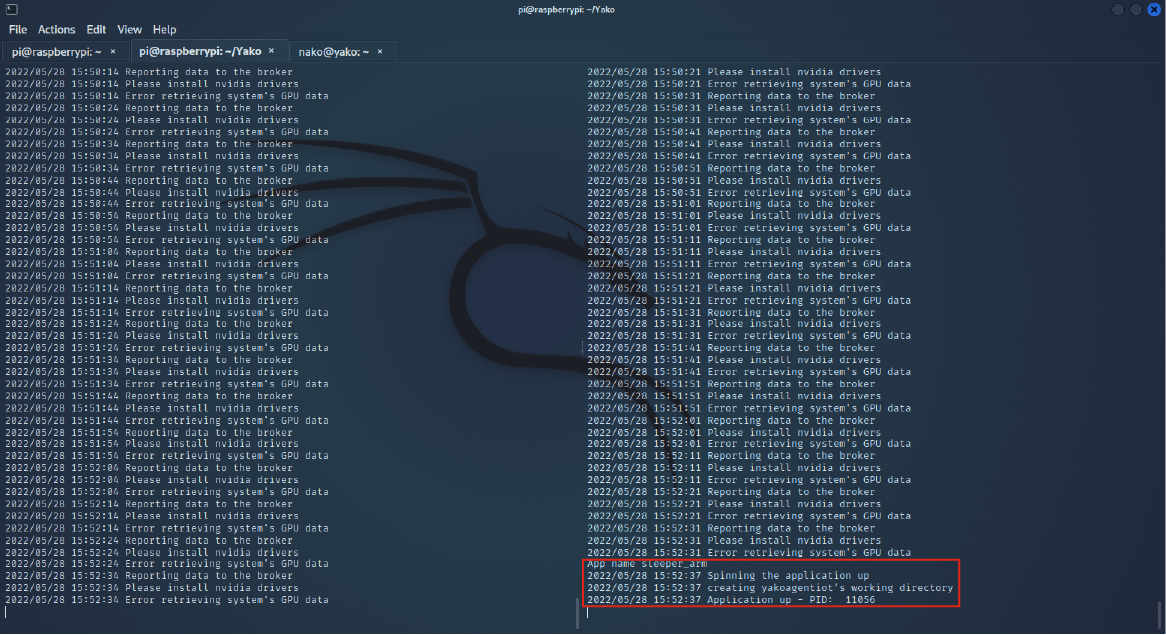
\includegraphics[width=\linewidth]{Results/test_iot_deploy.png}
                \caption{Deployed application to IoT device log}
                \label{fig:test_iot_deploy}
            \end{figure}
            
            The application was deployed correctly to the corresponding agent. The process was started on the node with PID: 11056.
            
            \begin{figure}[H]
                \centering
                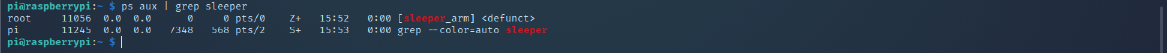
\includegraphics[width=\linewidth]{Results/test_iot_deploy_success.png}
                \caption{Deployed application to IoT device process}
                \label{fig:test_iot_deploy_success}
            \end{figure}
        
        \subsubsection{YakoAgent Application deployment}
            A slightly changed version of the previous sleeper program (see snippet \ref{code:sleeper}) was compiled as sleeper\_x86. Unlike the other, this version of the program will keep working until a kill signal is received. This application was dropped into the import box from the Upload Application page.
            
            \begin{code}
                \inputminted[
                    frame=lines,
                    framesep=2mm,
                    baselinestretch=1,
                    bgcolor=LightGray,
                    fontsize=\footnotesize,
                    escapeinside=||,
                    breaklines=true,
                    linenos
                ]{c}{Code/Results/sleeper.c}
                \caption{Sleeper }
                \label{code:sleeper}
            \end{code}
            
              In the system requirements form a node that was selected. The IoT Device checkbox was left unchecked. a summary of the requirements are illustrated in figure \ref{fig:test_agent_form_2}. The binary is then uploaded to the platform.
            
            \begin{figure}[H]
                \centering
                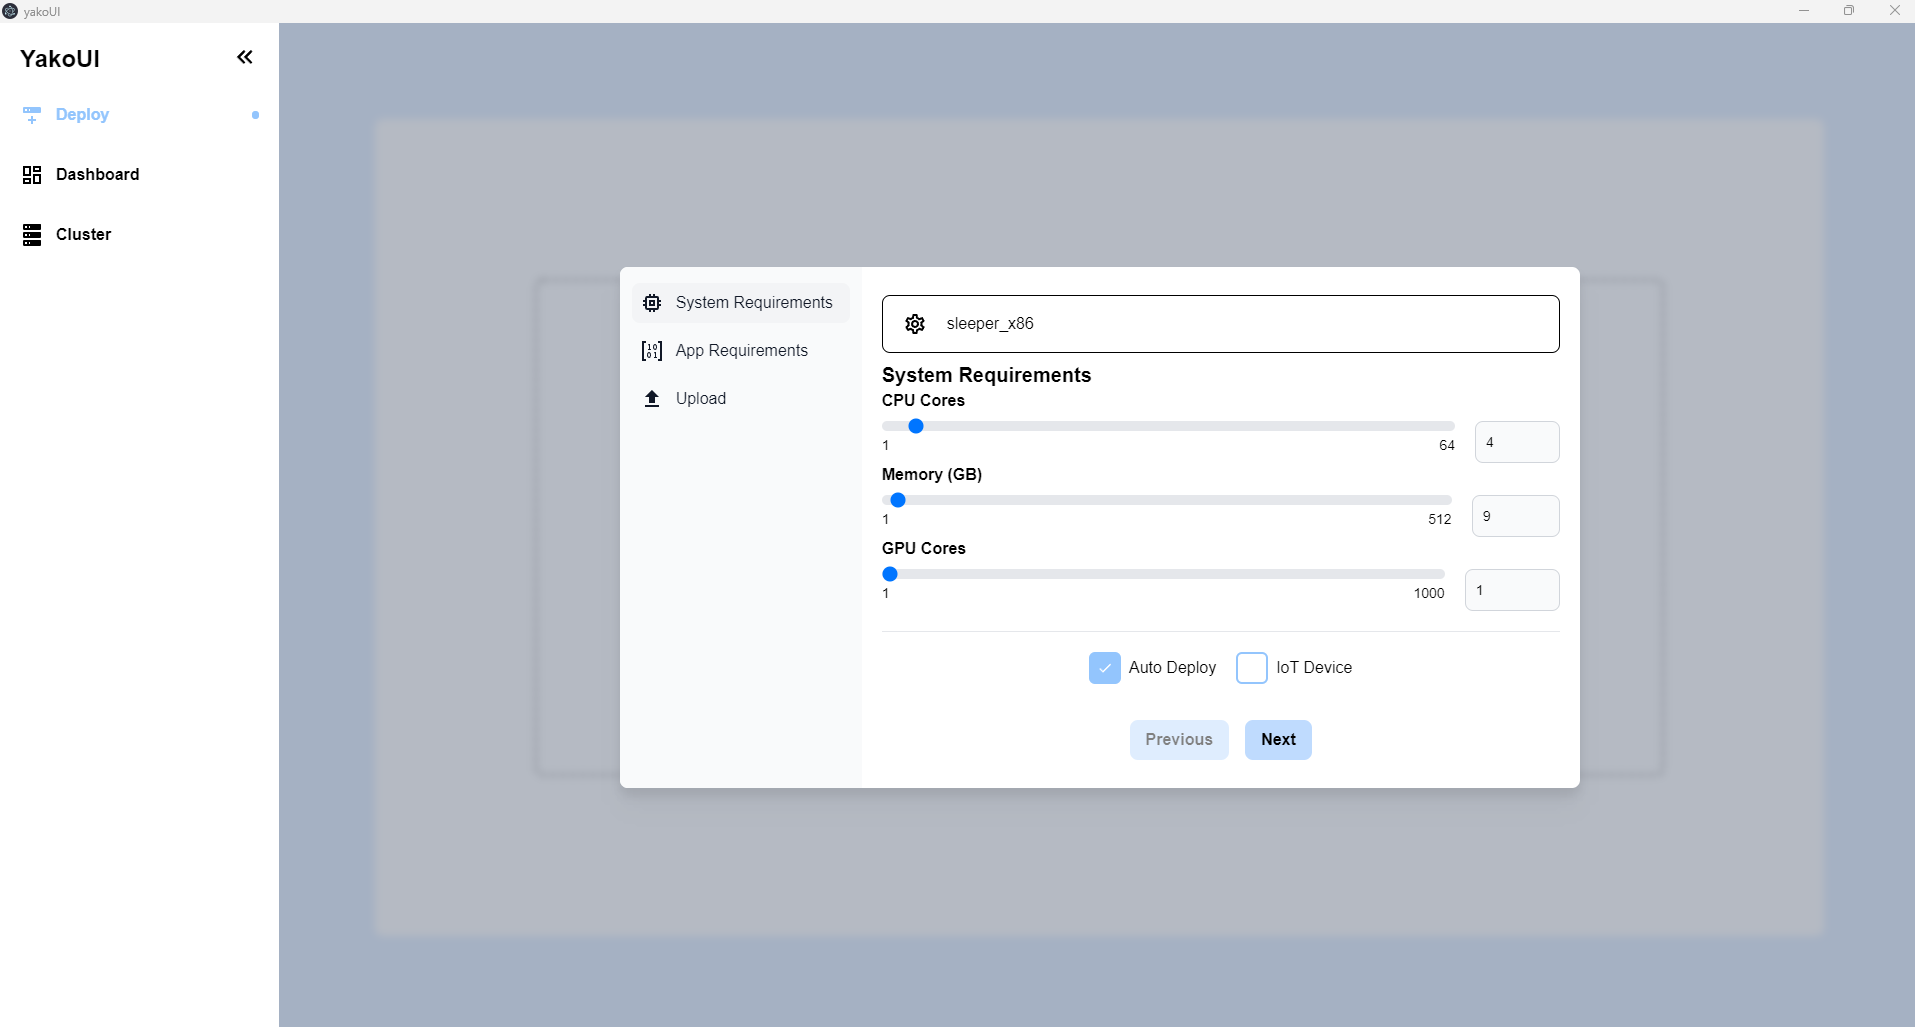
\includegraphics[width=0.8\linewidth]{Results/test_agent_form_1.png}
                \caption{System requirements form to deploy a 64-bits app to x86\_64 based devices}
                \label{fig:test_agent_form_1}
            \end{figure}
            
            \begin{figure}[H]
                \centering
                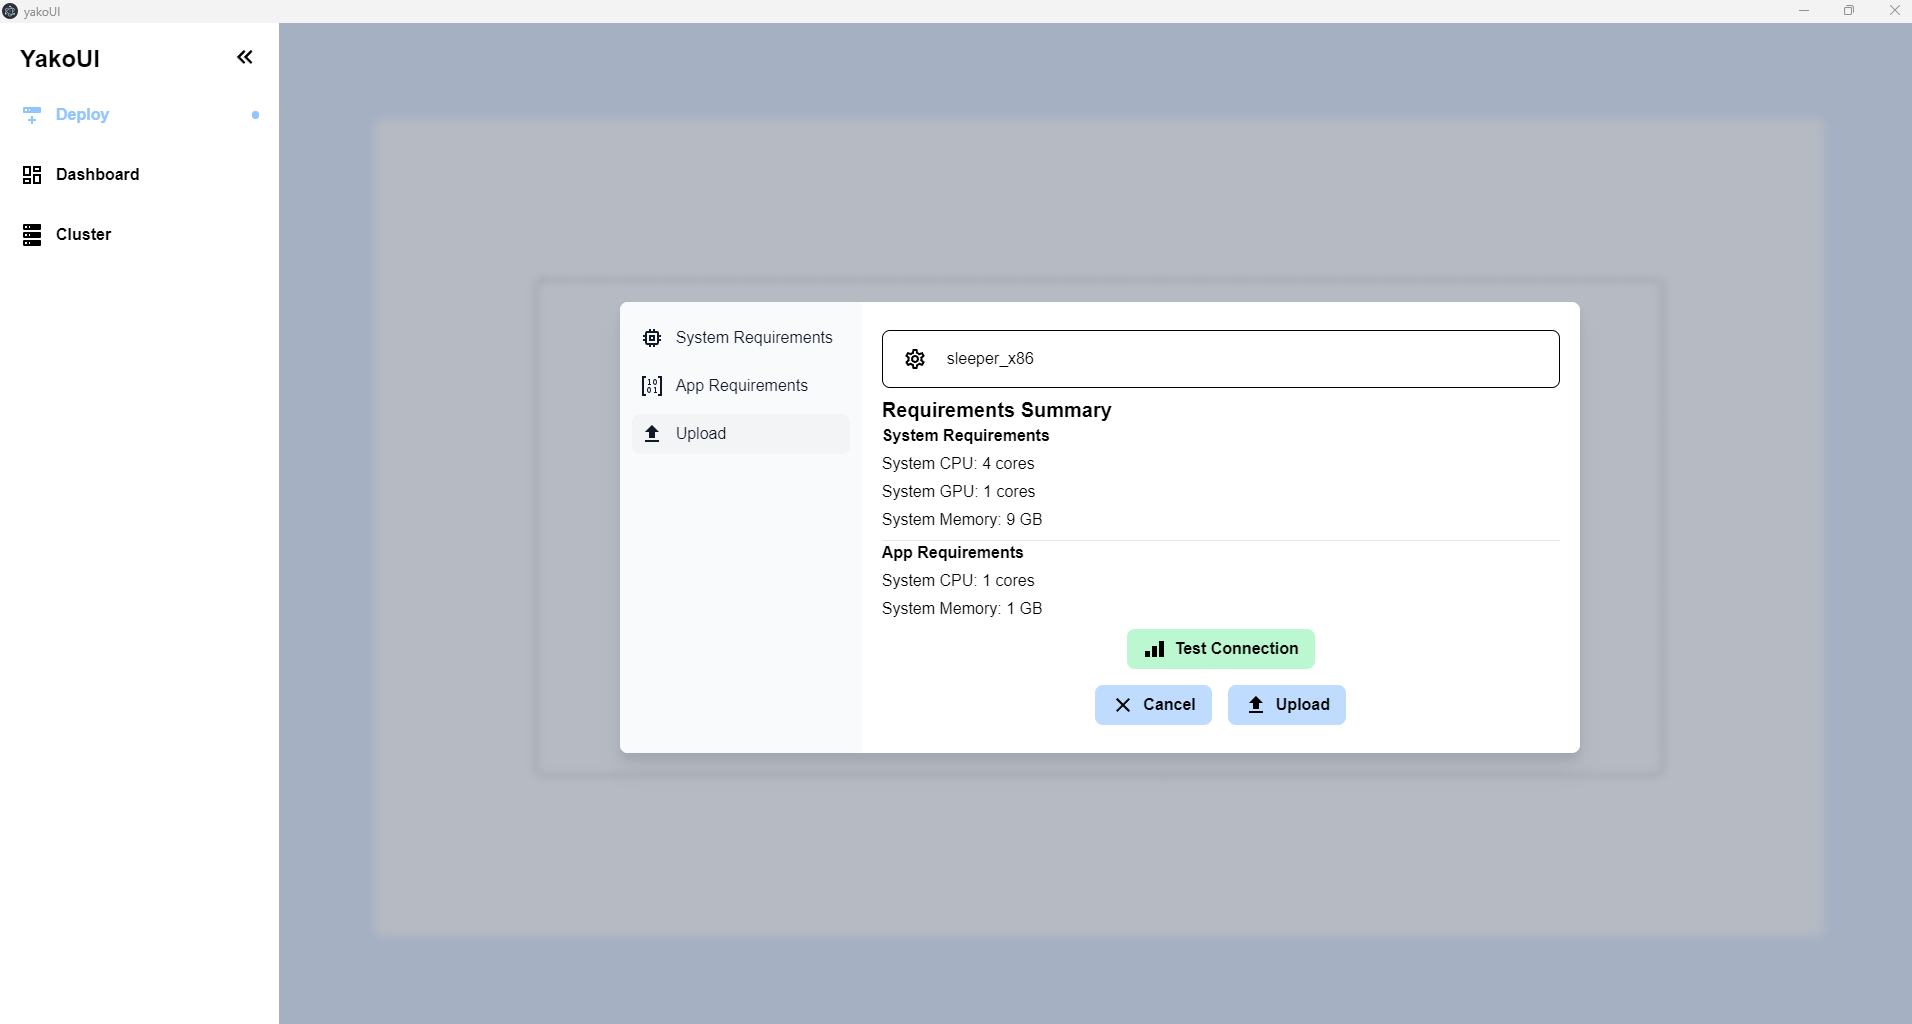
\includegraphics[width=0.85\linewidth]{Results/test_agent_form_2.png}
                \caption{Summarized deployment requirements}
                \label{fig:test_agent_form_2}
            \end{figure}
            
            
            On deployment request, the orchestrator will proceed to check the uploaded system requirements form and perform a search of the most suitable agent to deploy the application. In this test, IoT devices were discarded, and the agent selection was concluded among the remaining YakoAgents.
            The system requirements for this test was for the node to have 4 CPU cores and a total of 9GB of available free RAM. The application was finally deployed to YakoAgent n\_0000000324 which corresponds to the PC VM Yako4. As shown in the debugging and profiling picture \ref{fig:test_top_node_resources}, this node has a total of 4 CPU cores and 12GB of RAM allocated, of which $\mathtt{\sim}$10GB are available. It obtained a score of 2 brownie points, which positions the node as the most suitable one the run the app.
            
            \begin{figure}[H]
                \centering
                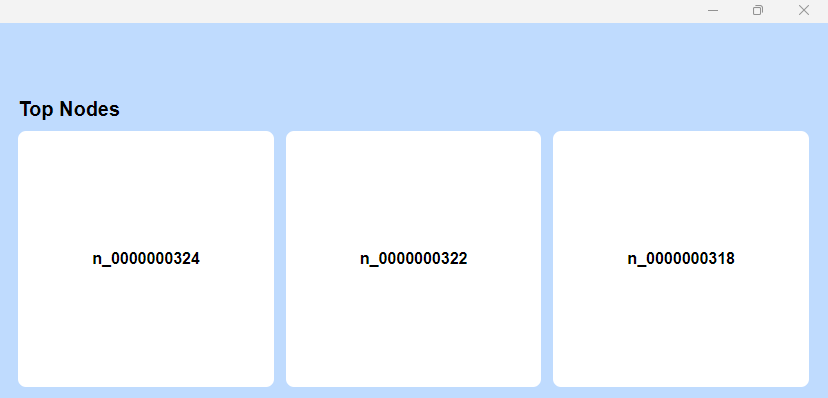
\includegraphics[width=0.75\linewidth]{Results/test_agent_top_nodes.png}
                \caption{Top 3 YakoAgents for the 64-bits app}
                \label{fig:test_agent_top_nodes}
            \end{figure}

            \begin{figure}[H]
                \centering
                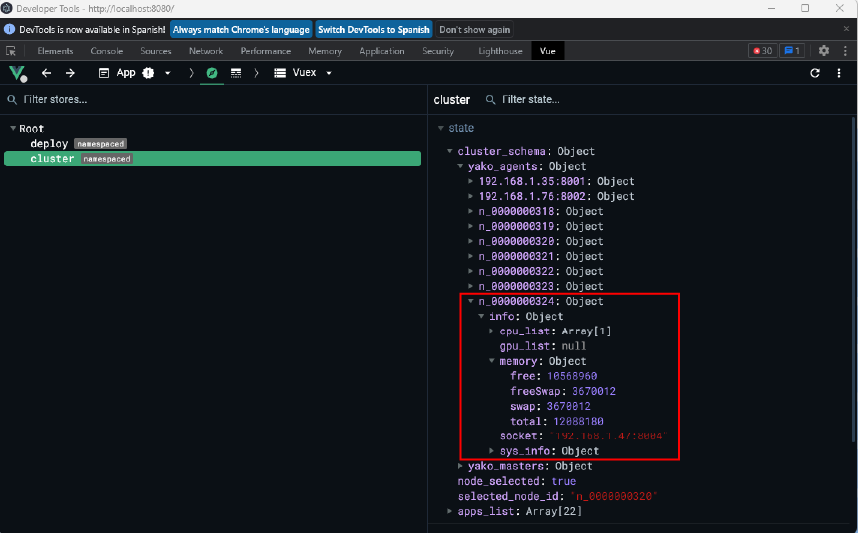
\includegraphics[width=\linewidth]{Results/test_top_node_resources.png}
                \caption{Top node system resources debug}
                \label{fig:test_top_node_resources}
            \end{figure}
            
            As illustrated in figure \ref{fig:test_agent_deploy}, the application was transmitted correctly via gRPC streaming. The software was also successfully started with PID: 3707. On the right terminal the process was shown after running a quick process search.
            
            \begin{figure}[H]
                \centering
                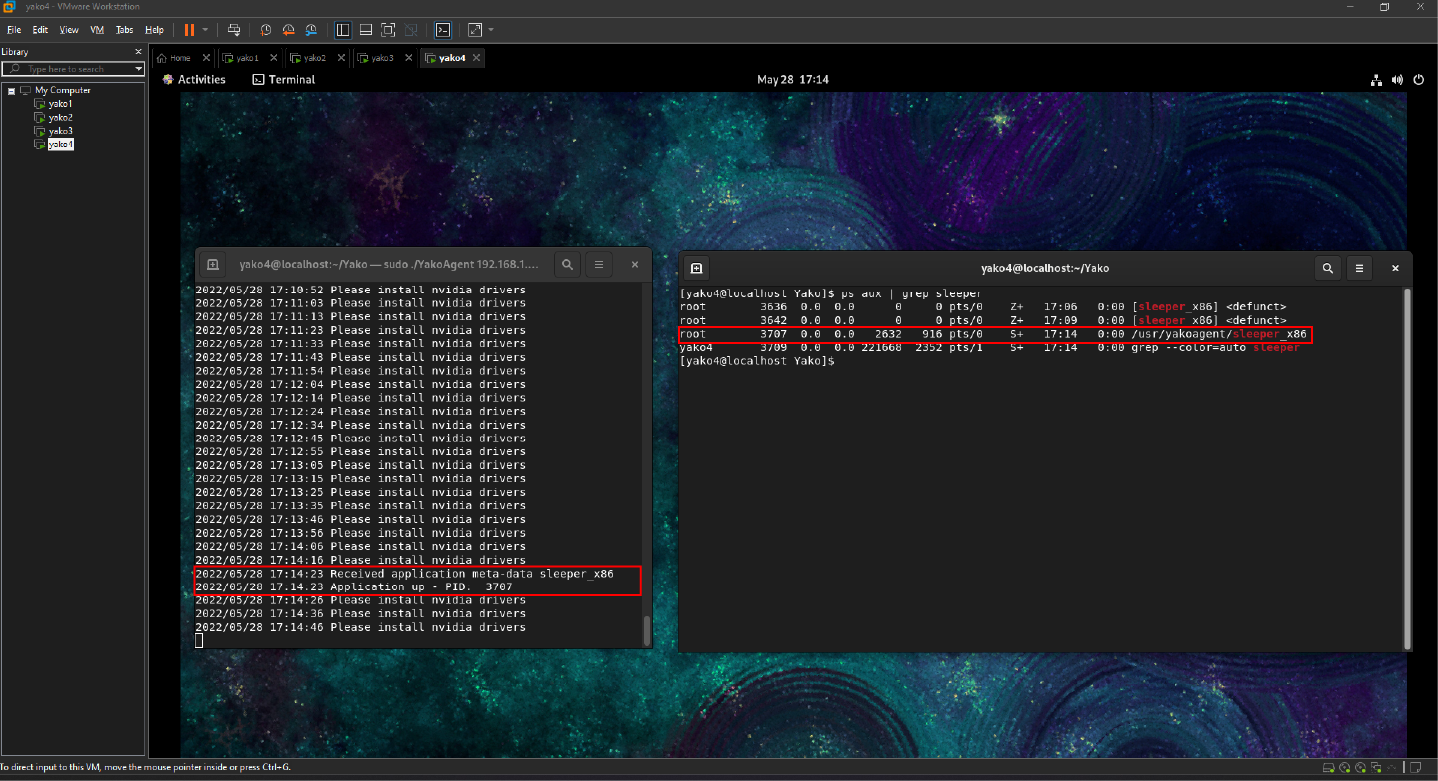
\includegraphics[width=\linewidth]{Results/test_agent_deploy.png}
                \caption{Deployed application to YakoAgent}
                \label{fig:test_agent_deploy}
            \end{figure}